\documentclass[12pt, a4paper]{article}

\usepackage{graphicx}
\usepackage{ragged2e}
\usepackage{multirow}
\usepackage{float}
\usepackage{enumerate}


\begin{document}

\title{Statistical Data Analysis: Bi-variate Data Analysis Project\\
\large Exploring the impact of temperature and precipitation on Crop Net Revenue}
\author{\textbf{Bushra Naeemi}
\\American University of Afghanistan
\\Instructor: Asadullah Jawid } 
\date{\today}
\maketitle 

\newpage
\tableofcontents

\newpage
\section{Introduction}
\justify
This Project is about finding the relationship or impact of temperature and rainfall on crop net revenue for the month of April by using correlation, co-variance, statistics, and graphical representations.
\section{Methodology}


\textbf{Measures of Central Tendency:} Mean\\
\textbf{Dispersion:} Standard Deviation and Range\\
\textbf{Distribution:} Skewness and Kurtosis\\
\textbf{Data tabulation:} Tables for organizing data.\\ 
\textbf{Co-variance} \\
\textbf{Correlation} \\
\textbf{Linear Model:} Intercept and slope.\\
\textbf{Summary: } R-squared.\\
\textbf{Graphical methods:}\\
\textbf{ }
\textbf {........Histogram}\\
\textbf {........Boxplot}\\
\textbf {........Density plot}\\ 
\textbf {........Scatter plot}\\

\newpage
\section{Results and Discussions}
\subsection{Descriptive Statistics of Variables}

\justify


\begin{table}[H]
\centering
\begin{tabular}{|r|r|r|r|r|r|r|}
  \hline
 Variables & Mean & S.Deviation & Min & Max & Skewness & Kurtosis \\
  \hline
  \hline
Temperature & 4.73 & 3.00 & 0.22 & 11.51 & 0.26 & -1.10 \\ 
  Rainfall & 60.02 & 27.84 & 28.93 & 123.62 & 0.85 & -0.68 \\ 
  Income(no.outlier) & 78369.58 & 287632.55 & -951500.00 & 7089500.00 & 14.15 & 279.70 \\ 
   \hline
\end{tabular}
\end{table}
\justify
\subsubsection{Temperature in April:} 

\begin{figure}[H]
\centering
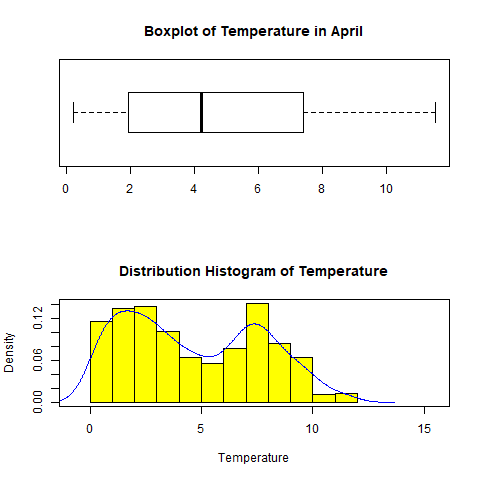
\includegraphics[trim={0 0 0 2cm}, scale=0.6, clip]{Temperature.png}
\caption{Distribution Graphs of Temperature}
\end{figure}

\justify
\textbf{Conclusion: }The average temperature in April ins 4.73 degrees, it's standard deviation is 3.00. which shows the distance of every variable to the mean and shows the distribution of temperature data. It's value is between the range of 0.22 and 11.51. The more the value of skewness departs from zero (in either directions), the more the distribution is getting skewed (to the left (long tail at the left), or right(long tail to the right)). So our data is close to normal and a little skewed to the right side. The value of kurtosis -1.10, indicates lighter tails than normal (thinner than normal)   (See Figure 1)

\justify
\subsubsection{Rainfall in April:}

\begin{figure}[H]
\centering
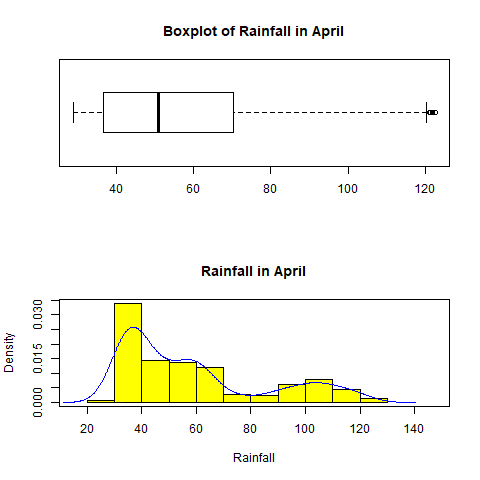
\includegraphics[trim={0 0 0 2cm}, scale=0.6, clip]{RainFall.png}
\caption{Distribution Graphs of Rainfall}
\end{figure}

\justify
\textbf{Conclusion: }  The average rainfall in April is 60.02, standard deviation is 27.84. It's rage is between 28.93 and 123.62. the skewness value 0.85 shows that the graph is skewed to the right side, the kurtosis value -0.68 shows that it is lighter tail than normal.(See Figure 2) 
\newpage
\justify
\subsubsection{Crop Net Income of Farms in April:}

\begin{figure}[H]
\centering
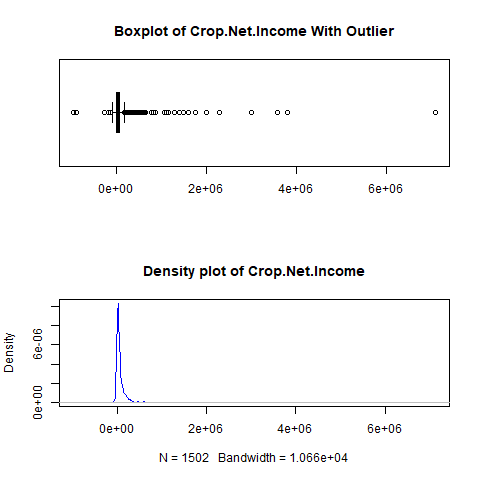
\includegraphics[trim={0 0 0 2cm}, scale=0.5, clip]{Income.png}
\caption{Distribution of crop net income with outliers}
\end{figure}

\justify
\textbf{Note: } The Crop Net Income has a large number of outliers that should be removed from the data, to make effective conclusions.

\begin{figure}[H]
\centering
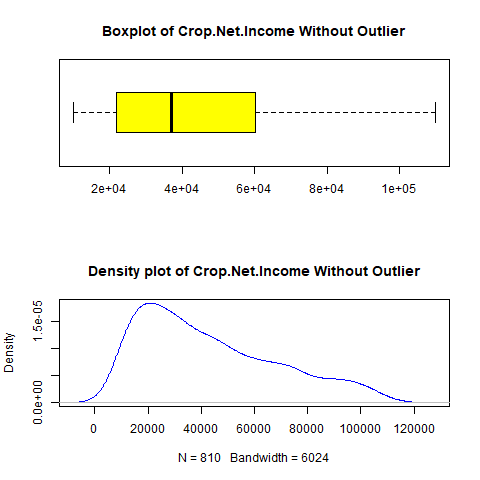
\includegraphics[trim={0 0 0 2cm}, scale=0.5, clip]{income2.png}
\caption{Distribution of crop Net Income Without Outliers}
\end{figure}

\justify
\textbf{Conclusion: } This is the graphs of crop net income without outliers, now the mean can be considered as central point for this graph. The average of crop net income in April is 78369.58, with standard deviation of 287632.55. It's range is between -951500.00 to 7089500.00. the skewness value 14.15 shows that the data has been skewed to the right side, and the kurtosis of 279.70 shows that the graph has heavier tails than normal or it is flatter than normal. (See figure 4)

\subsection{Bi-Variate Statistical Data Analysis}
\subsubsection{Association of Temperature and Crop Net Income in April}

\begin{table}[h]
\begin{center}
\caption{Results of Temperature and Crop Net Income in April}
\begin{tabular}{|c|c|c|r|l|}
	\hline
     \multirow{2}{*}{Variables} & Co-variance & Correlation & 
     Linear Model & R-Squared \\ & & & Intercept/Slope & \\
     \hline
     \hline
     Temperature/C.income  &1001.831 & 0.0128 & 42494.7 /106.6   & 0.0001637 \\
     \hline
\end{tabular}
\end{center}
\end{table}
\justify
\textbf{Co-variance:} Co-variance of temperature and crop net income is 1001.831, the positiveness of co-variance shows the positive linear relationship. When one variable increases/decreases the second variable does too. \\
\\
\textbf{Correlation:} The correlation of temperature and crop net income is 0.0128, so their relationship is weak, and don't have so much impact on each other.\\
\\
\textbf{Linear Model: } 

\item \textbf The positive slope of 106.6 shows that crop net income is dependent upon temperature. For every unit of increase in temperature, crop net income is expected to increase by 106.6 units.


\justify
\textbf{R-Squared}: 
The value of 0.0001637 means that 0.01\% of the crop net income(dependent variable) is explained or effected by temperature(independent variable).

\begin{figure}[H]
\centering
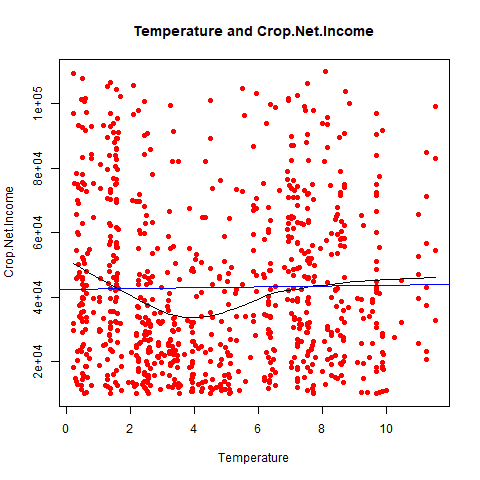
\includegraphics[trim={0 0 0 0}, scale=0.7, clip]{temperature_Income.png}
\caption{Association of Temperature and Crop Net Income in April}
\end{figure}

\justify
\textbf{Conclusion:} We can see from scatter plot   that  both temperature, and crop net income increases in relation to on another, which is  positive slightly rising linear line in our graph.The correlation of 0.0128 shows a weak positive relationship between temperature and crop net income.  (See figure 5)  \\
\newpage
\subsubsection{Association of Rainfall and Crop Net Income in April}

\begin{table}[h]
\begin{center}
\caption {Association of Rainfall and Crop Net Income}
\begin{tabular}{|c|c|c|r|l|}
	\hline
     \multirow{2}{*}{Variables} & Co-variance & Correlation & 
     Linear Model & R-Squared \\ & & & Intercept/Slope & \\
     \hline
     \hline
     Rainfall/Income  & -197568.1 & -0.291143 & 59404/-280 & 0.08476 \\
     \hline

\end{tabular}
\end{center}
\end{table}

\justify
\textbf{Co-variance:} Co-variance of rainfall and crop net income is -197568.1, the negativeness of co-variance shows the negative linear relationship. When one variable increases the second variable decreases and vice versa.\\
\\
\textbf{Correlation:} The correlation of temperature and crop net income is -0.291143, so their relationship is weak because it's between the range of -0.5 and 0.5. And have 29\% impact on each other. \\
\\
\textbf{Linear Model: } 

\item \textbf The negative slope of -280 shows that crop net income is dependent upon rainfall. For every unit of increase in rainfall, crop net income is expected to decrease by -280 units. 


\justify
\textbf{R-Squared}: The value of 0.08476 means that 8.4\% of the crop net income is explained by rainfall.

\begin{figure}[H]
\centering
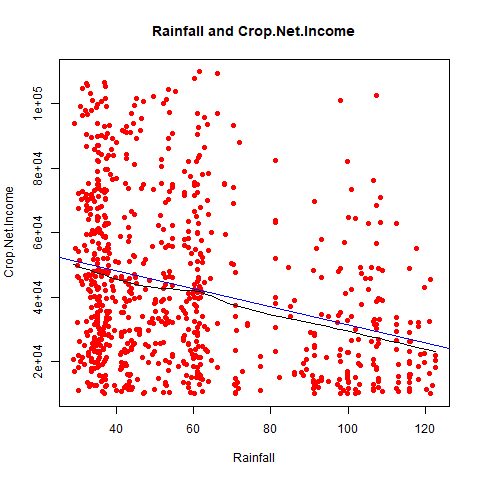
\includegraphics[trim={0 0 0 0}, scale=0.7, clip]{rainfall_Income.png}
\caption{Association of Rainfall and Crop Net Income}
\end{figure}

\justify
\textbf{Conclusion:} The negative correlation of -0.291143 shows a weak negative linear relationship among rainfall and crop net income. Means that 0.29\% of variation in crop net income is explained by rainfall. By increase of rainfall crop net income decreases.(See figure 6) \\

\section{Summary}
\textbf{Summary: }\\
Our data is about finding the relationship between temperature, rainfall, and crop net income. As we can see temperature and crop net income have direct linear relation, by increasing in the value of temperature, the crop net income increases too. It means the more the temperature the more revenue farmers make. But the impact of temperature is very less on income. But the relationship of rainfall and crop net income is indirect. The more the rainfall the less the income of farm. But still it doesn't have a lot of impact on income. 0.29\% of variation in crop net income is explained by rainfall.  



\end{document}